
\documentclass{article}
\usepackage{hyperref}
\usepackage{fontspec}
\usepackage{graphicx}
\usepackage{url}
\usepackage{fancyhdr}
\usepackage{titling}

\fancypagestyle{unicodeproposal}{%
\fancyhf{} % clear all header and footer fields
\rhead{Page \thepage} % except the center
\lhead{\thetitle}
}

\pagestyle{unicodeproposal}

\setmainfont{Times New Roman}
 
\begin{document}
\title{Lemur Emoji Submission}
\author{Huáng Jùnliàng, Yè Wéi}
\begin{titlepage}
  \centering
  \vfill
  \vfill
  
\includegraphics[scale=1]{lemur.png}
  \vskip 1.5cm
  {\bfseries\Large
    \thetitle
  }
  \vskip 1.5cm
  {
    \theauthor
    \vskip 1.2ex
    \today
    \\
  }
  \vskip 4cm
  \vfill
\end{titlepage}

\begin{abstract}
    We are proposing the addition of LEMUR Emoji. It would represent a visually distinct primate animal in Madagascar. Emoticons that feature lemur have already existed, such as iMessage and Line stickers, suggests certain level of interest in lemur emoji.
\end{abstract} 

\section{Introduction}
Lemurs (\textit{Lemuroidea}) are a clade of primates endemic to the island of Madagascar. They have large, round reflective eyes, wailing screams. They also have furry, pointed ears and long tails. Being the most wildly recognized primate, the ring-tailed lemur, known as maky in Malagasy language, has been selected as the symbol for Madagascar National Parks and considered as an icon of Madagascar.

The Unicode has encoded some significant primates, i.e. Monkey, Gorilla, including Lemur will help completing the set. Lemur is visually distinct and it cannot be represented by current mammals emoji.

While lemurs are traditionally protected due to their resemblance to humans, because of which they are revered as a symbol of ancestors in some regions, the IUCN considers them to be the world's most endangered mammals, noting that as of 2013 up to 90\% of all lemur species face extinction within the next 20 to 25 years\footnote{``Lemur": \url{https://en.wikipedia.org/wiki/Lemur}}. A lemur emoji can help people recognize the risk of extinction and the conservation efforts.

% Lemurs' cute appearances and rareness making them a unique attraction for foreign travellers till this day. 
% And they have also become a popular African element in Western films and videos during the past 20 years. 
% For example, the original 2005 animated film Madagascar was seen by an estimated 100 million people in theaters and 200–300 million people on DVD worldwide.
% Prior to this movie, Zoboomafoo, a Public Broadcasting Service (PBS) children's television series from 1999 to 2001,
% helped to popularize sifakas by featuring a live Coquerel's sifaka from the Duke Lemur Center as well as a puppet.
% A twenty-episode series called Lemur Kingdom (in the United States) or Lemur Street (in the United Kingdom and Canada) aired in 2008 on Animal Planet. 
% It combined the typical animal documentary with dramatic narration to tell the story of two groups of ring-tailed lemurs at Berenty Private Reserve.(from wiki)

\section{Identification}
\subsection{CLDR Short Name}
lemur

\subsection{CLDR keywords}
maky | Madagascar

\section{Sample images}

\begin{figure}[h]
  
\includegraphics{lemur.png}
\end{figure}

Source: \url{https://pngimg.com/download/61776}

License: CC-4.0-BY-NC

\section{Selection Factors -- Inclusion}
\subsection{Compatibility}
No compatibility factors.

\subsection{Expected usage level}
\subsubsection{Frequency}

Google Trends (Figure \ref{fig:google-trend}) shows a consistent search interest in ``lemur" in the past year, though it is significantly lower than the one in ``elephant" or ``monkey".

\begin{figure}[h]
  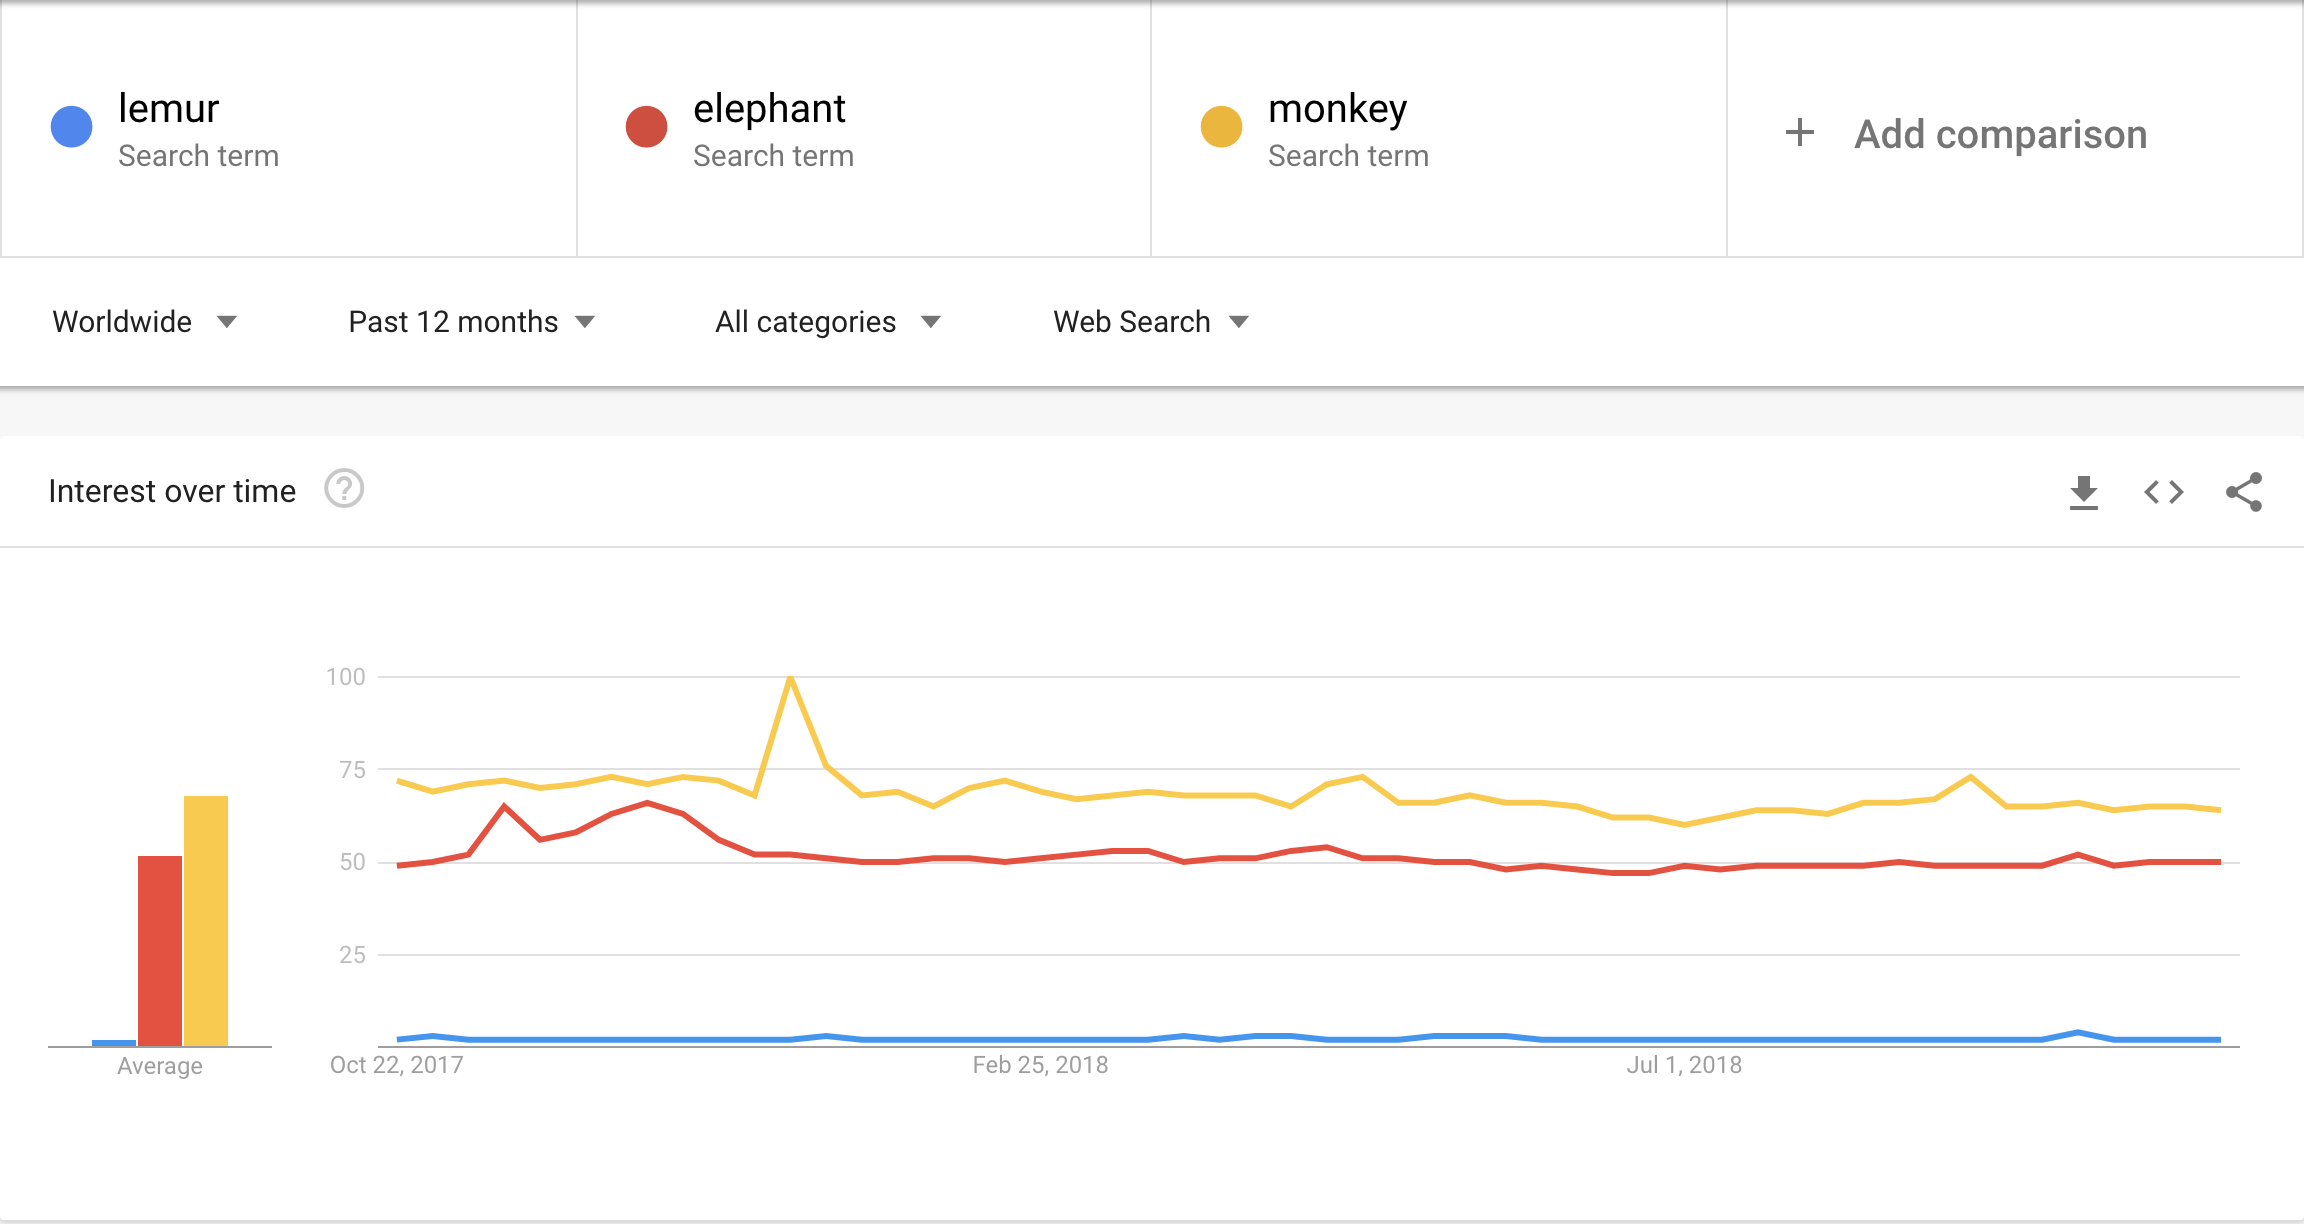
\includegraphics[width=\linewidth]{img/google-trend.png}
  \caption{Google Trends show interest over time on three terms: ``lemur", ``elephant" and ``monkey".}
  \label{fig:google-trend}
\end{figure}

Google Ngram Charts (Figure \ref{fig:google-ngram}) shows the word ``lemur" is of relatively lower occurrence in printed books compared with ``elephant" and ``monkey".

\begin{figure}[h]
  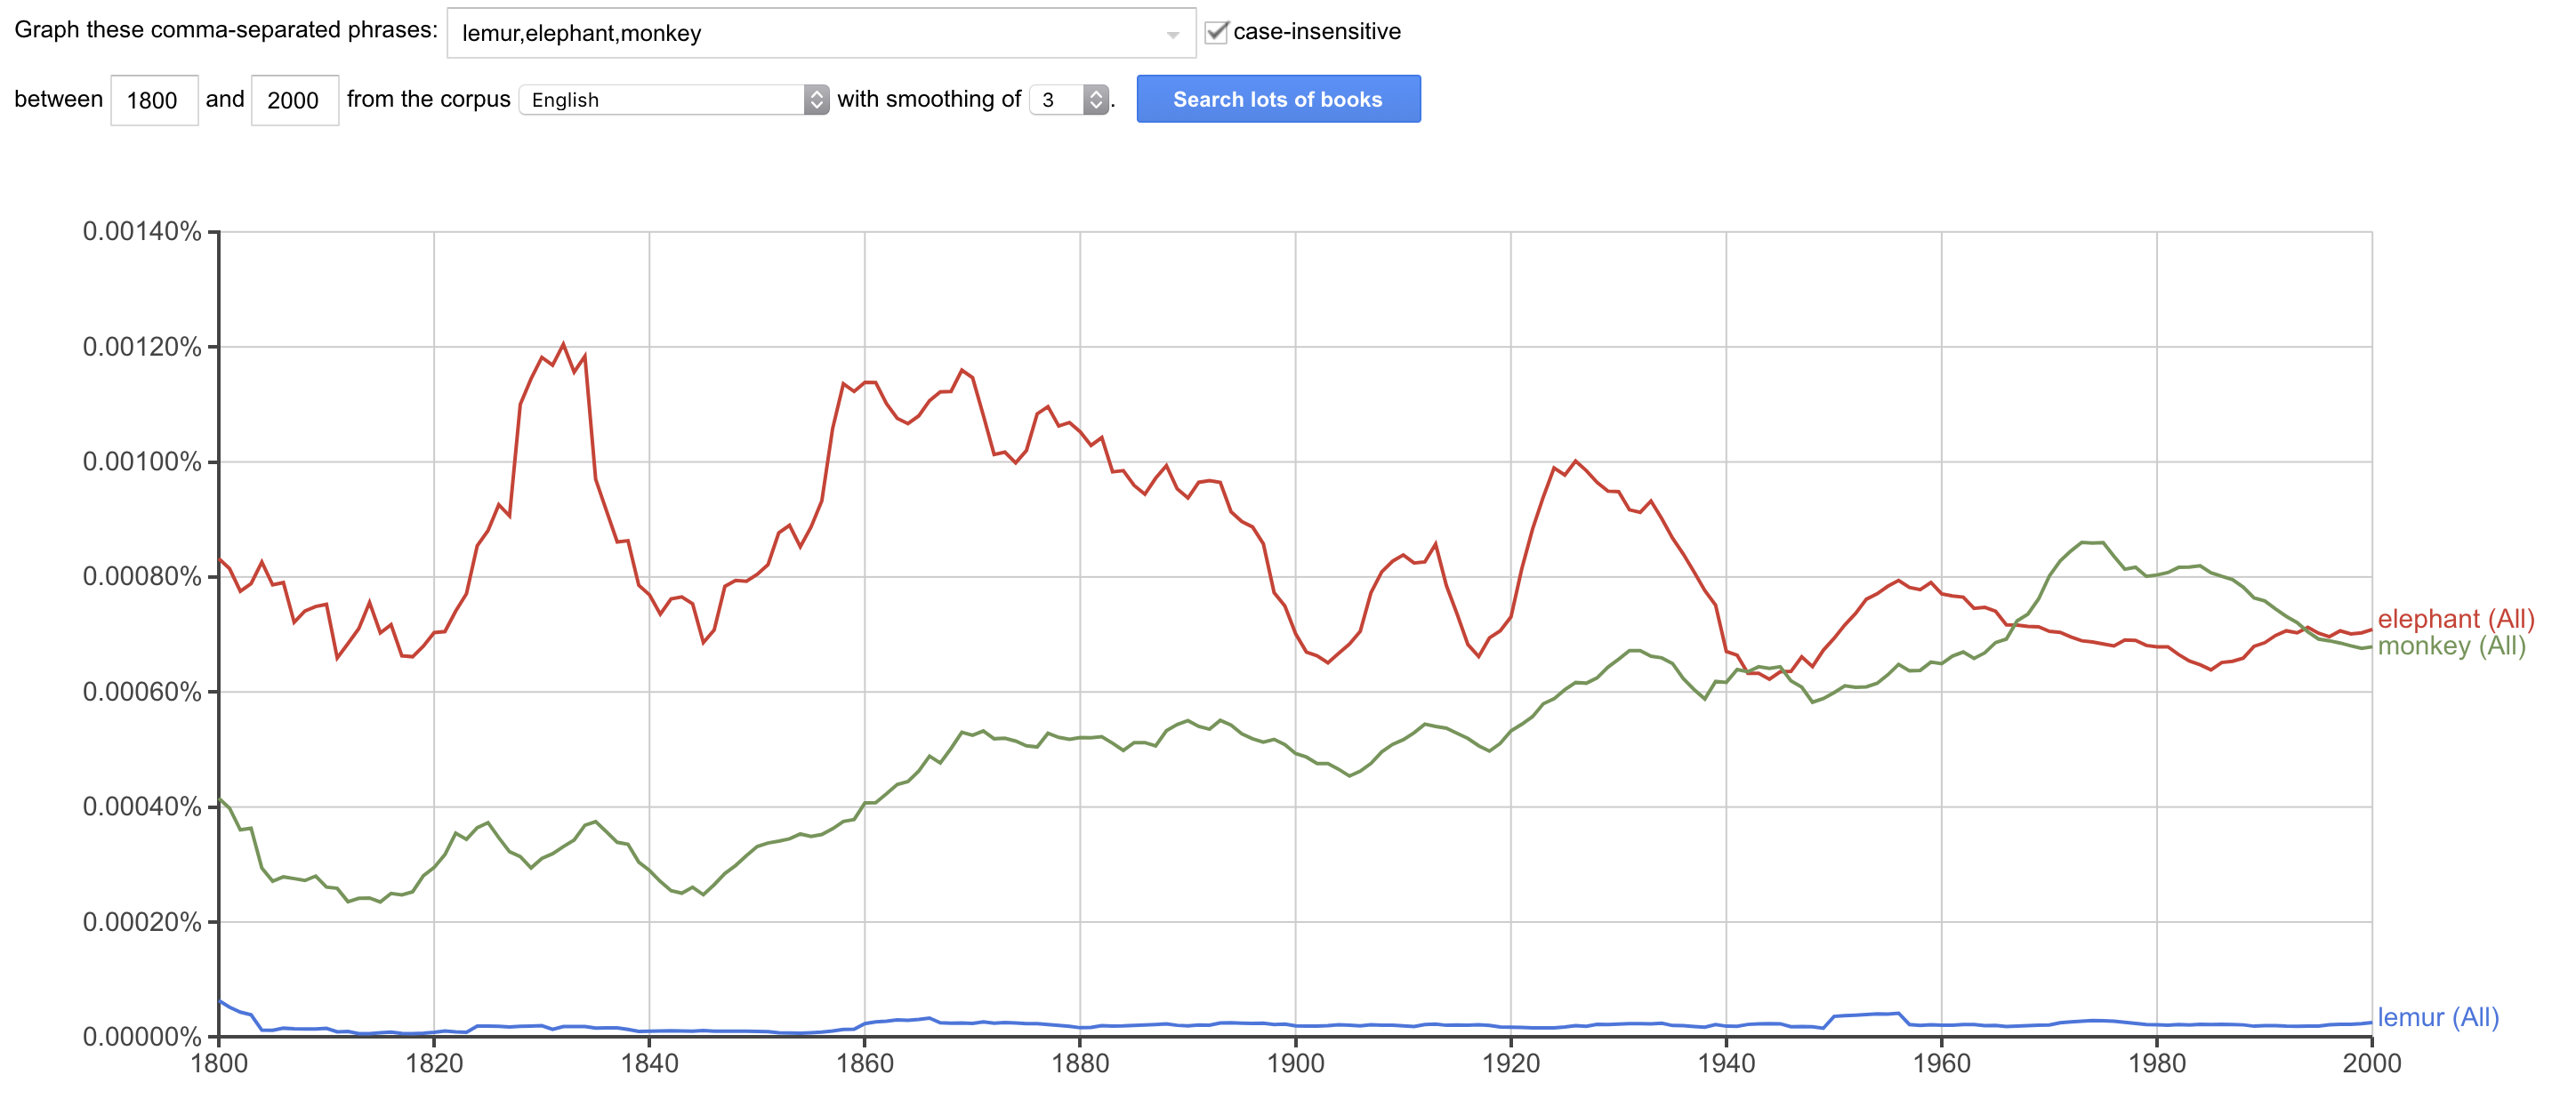
\includegraphics[width=\linewidth]{img/google-ngram.png}
  \caption{Google Ngram Charts on three words: ``lemur", ``elephant" and ``monkey".}
  \label{fig:google-ngram}
\end{figure}

Besides, we can also measure the popularity of Lemur in readers by checking the pageviews analysis of Wikipedia (Figure \ref{fig:wikipedia-pageviews}). Again we compare ``lemur" with ``elephant" and ``monkey".

\begin{figure}[h]
  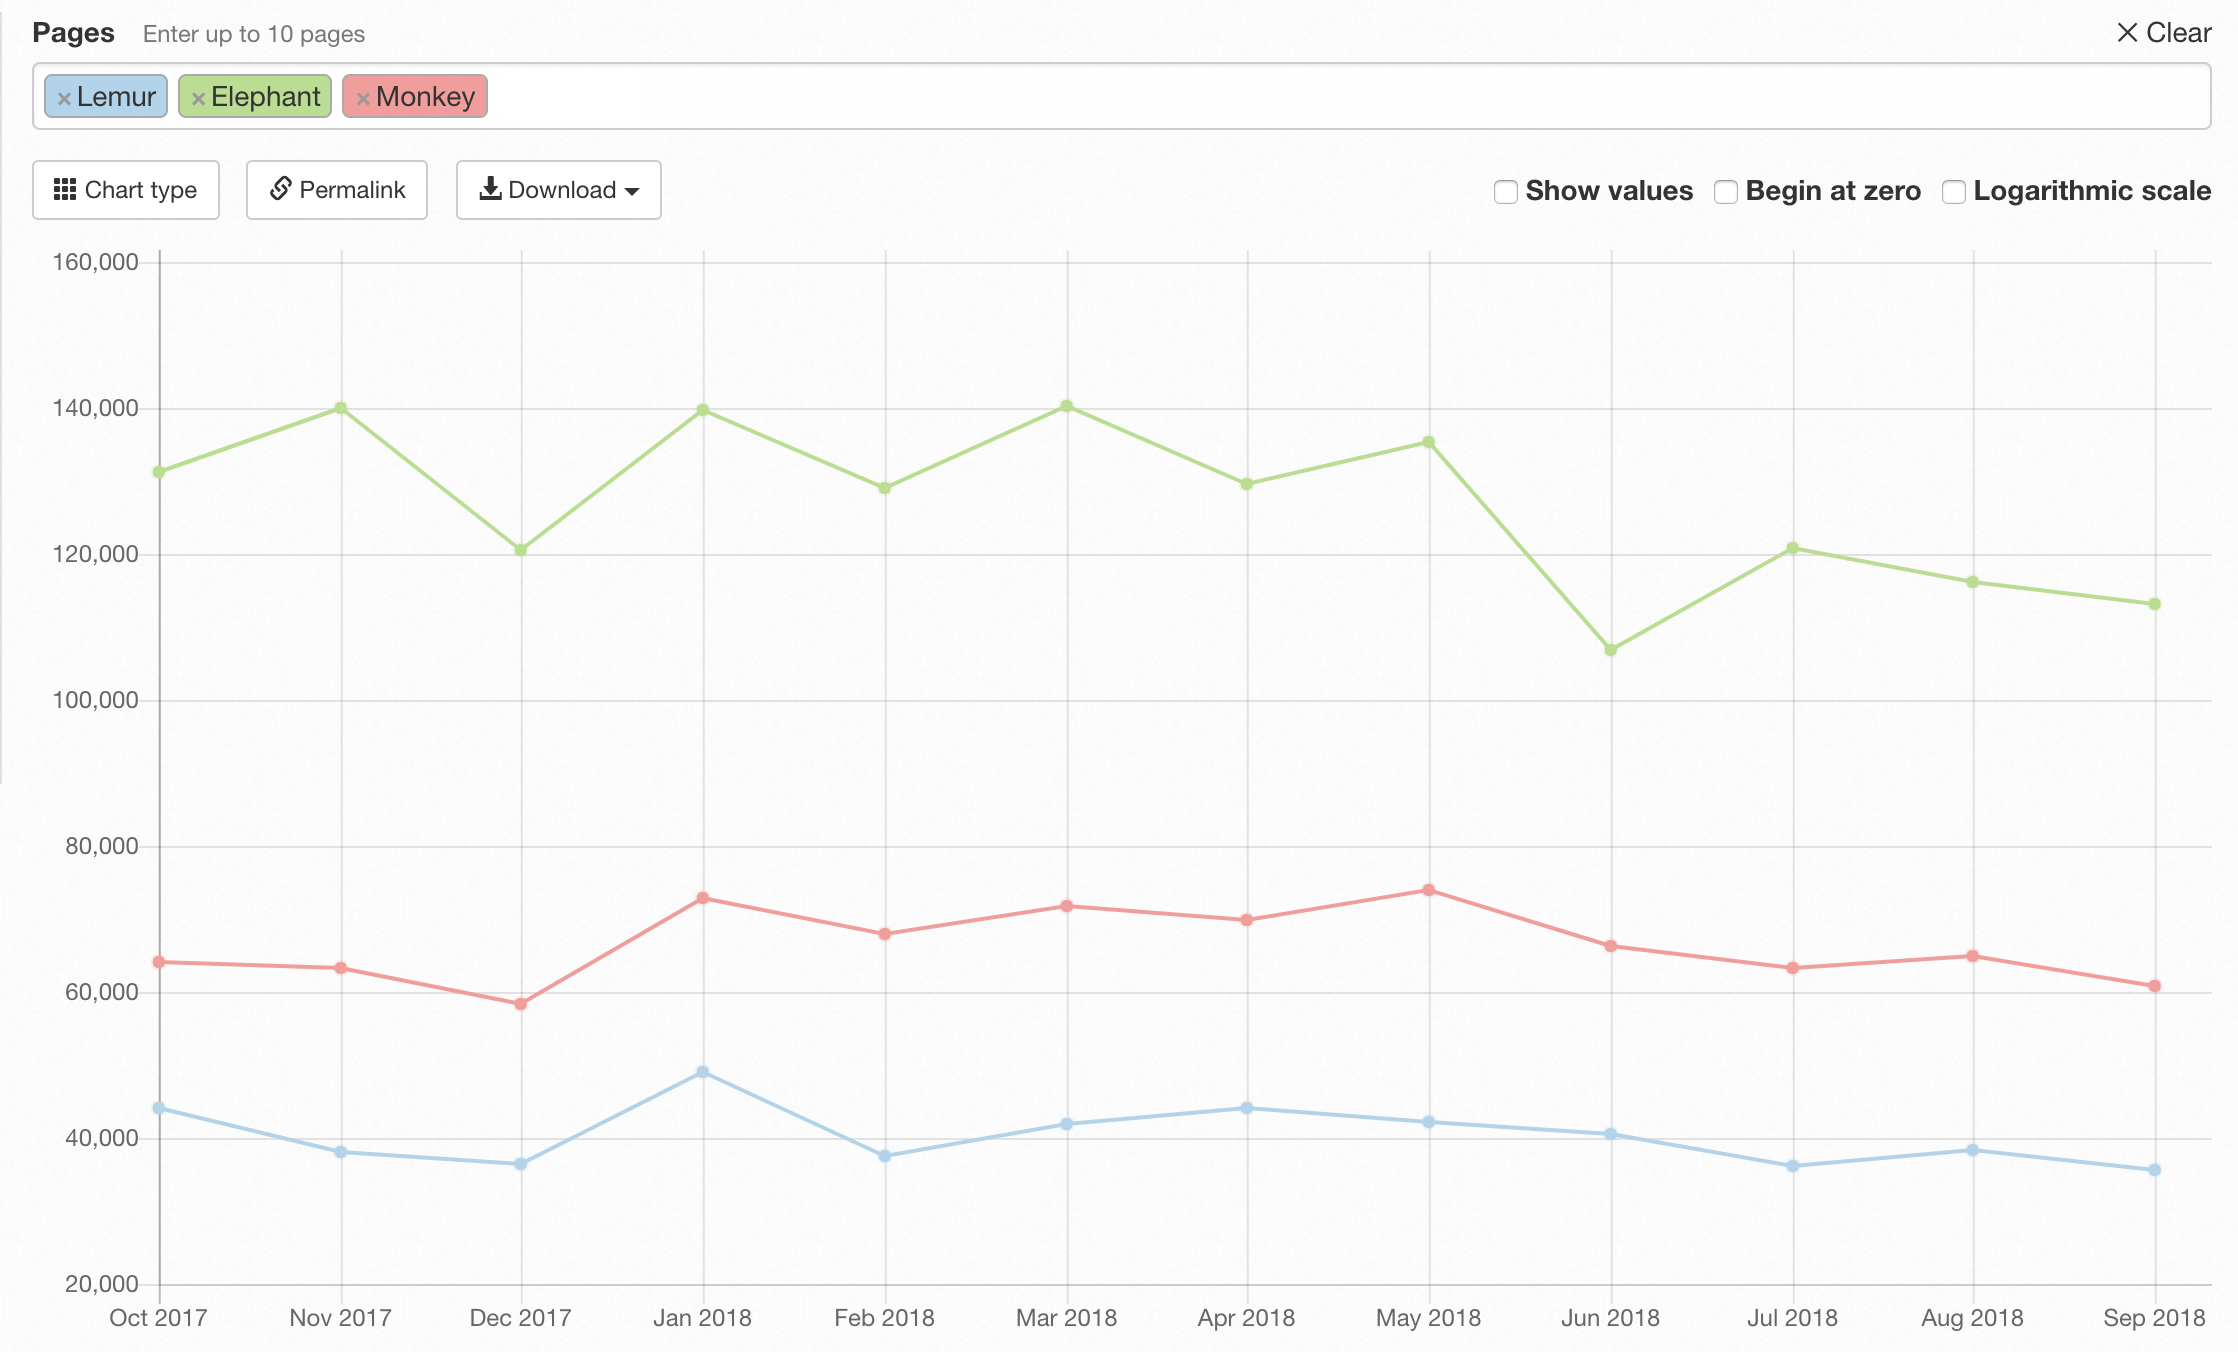
\includegraphics[width=\linewidth]{img/wikipedia-pageviews.png}
  \caption{Wikipedia pageviews on three pages: ``lemur", ``elephant" and ``monkey".}
  \label{fig:wikipedia-pageviews}
\end{figure}

As show on the figure, over the past year, the article on Lemur has accumulated 480,000 pageviews, which is also consistently proportional to the ones of article on monkey. The statistics shows a strong and lasting interest among the internet users to Lemur.

\subsubsection{Multiple Usages}
For symbolism, Indri, one species of lemur, is known as little father. Its large size and upright walking posture resembles to human and their ancestors. Some regions believes that human begins with indri and reveres it as a clan.\footnote{``Lemur are cultural creatures": \url{https://www.lemurreserve.org/wp-content/uploads/2017/06/18\_Lemurs\_are\_Cultural\_Creatures\_4-5.pdf}}

\subsubsection{Use in sequences}
n/a

\subsubsection{Breaking new ground}
No. Lemur emoji helps complete the current mammals emoji set.

\subsection{Image distinctiveness}
Lemur is distinctive in their long, black and white ringed tail, a different coloring to MONKEY. Despite the similar striped tail coloring, 
their slender frame, narrow face and fox-like muzzle differentiate it from RACOON.
In all, it is visually unlike any other current mammals emoji.

\subsection{Completeness}
Lemur fills a gap in emoji for well-known distinct primates endemic in Madagascar and also a symbol of ancestors.

\subsection{Frequently requested}
Yes. A lemur emoji is frequently requested on Twitter from time to time (Figure \ref{fig:request-lemur-evidence-tweet}).

\begin{figure}
    
\includegraphics[width=\linewidth]{img/request-lemur-evidence-tweet-1.png}
    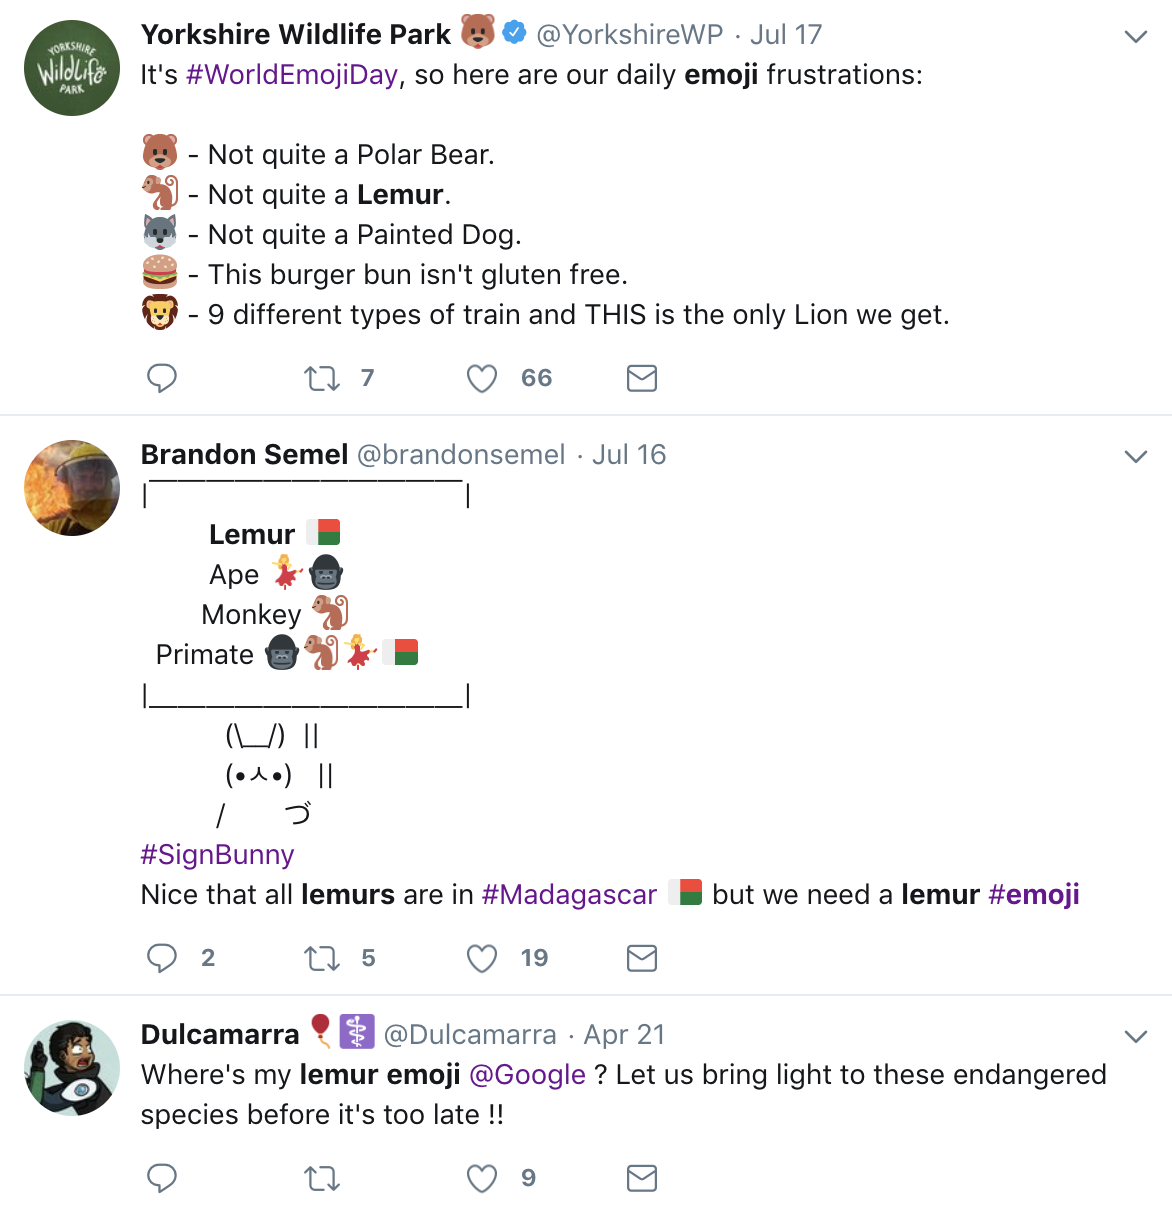
\includegraphics[width=\linewidth]{img/request-lemur-evidence-tweet-2.png}
    \caption{Users request lemur emoji on Twitter}
    \label{fig:request-lemur-evidence-tweet}
  \end{figure}

Instagram \footnote{``\#lemur hashtag on Instagram": \url{https://www.instagram.com/explore/tags/lemur/}} has 315,267 posts tagged \#lemur.

To meet the user request, there are vendors offering lemur sticker on different communication platforms. iOS App Store has 9 iMessage lemur sticker sets and Line Store has 33 lemur sticker sets\footnote{``Results for `lemur' in LINE stickers": \url{https://store.line.me/search/en?q=lemur}}. This implies that there are quantifiable numbers of people interested in using lemur stickers. However, these stickers are proprietary to each platform and thus it is not compatible to other platforms. If we can have lemur as a Unicode emoji, these compatibility issues can be averted.

\section{Selection Factors -- Exclusion}
\subsection{Overly specific}
Not overly specific. Lemur is of same level of specificity of other animal-mammal ones in its category. It refers to one family of animal, rather
than being too specific, because no other type of lemur emoji exists at this time.

\subsection{Open-ended}
No. Lemur is distinct.

\subsection{Already representable}
No. Some twitter users has resorted to use MONKEY emoji (Figure \ref{fig:monkey-emoji-substitute-tweet}) or MONKEY, FOX FACE ``sequence" (Figure \ref{fig:fox-face-monkey-emoji-substitute-tweet}) as a substitute, but this is not acceptable and may cause misinterpretation if lack of written explanation.

\begin{figure}
  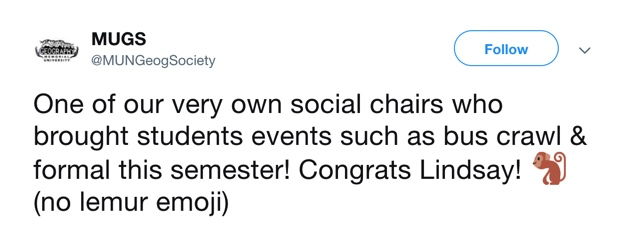
\includegraphics[width=\linewidth]{img/monkey-emoji-substitute-tweet.jpg}
  \caption{Using monkey to represent for lemur and explanation\protect\footnotemark}
  \label{fig:monkey-emoji-substitute-tweet}
\end{figure}
\footnotetext{\url{https://twitter.com/MUNGeogSociety/status/854678060209197056}}

\begin{figure}
  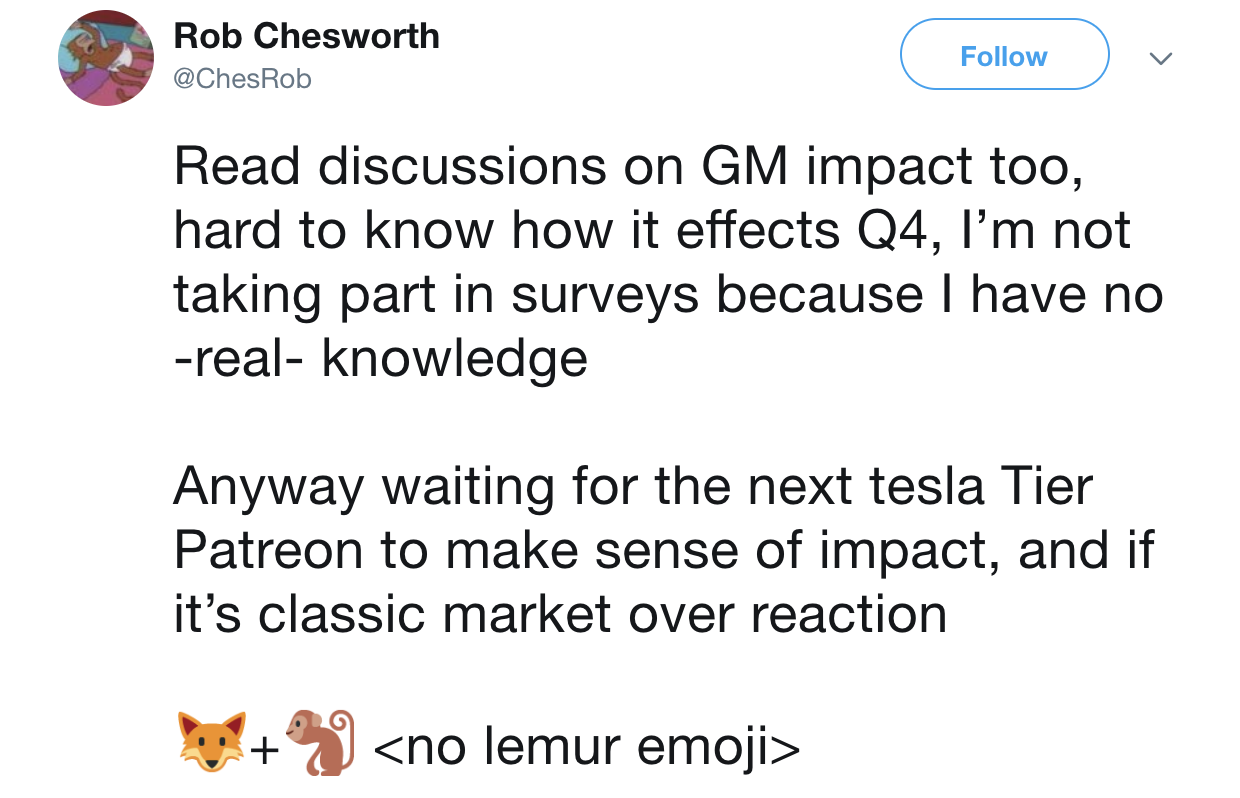
\includegraphics[width=\linewidth]{img/fox-face-monkey-emoji-substitute-tweet.png}
  \caption{Using fox face and monkey ``sequence" to represent for lemur and explanation\protect\footnotemark}
  \label{fig:fox-face-monkey-emoji-substitute-tweet}
\end{figure}
\footnotetext{\url{https://twitter.com/ChesRob/status/1053395209910927362}}

\subsection{Logos, brands, UI icons, signage, specific people, deities}
The Maki Company's logo\footnote{``Maki": \url{http://maki-company.com/index.php}} portrays the face of sifaka, a species of Lemurs. Lemur is also selected as the symbol of Madagascar National Parks. Besides, lemur are mostly used for non-profit organizations on lemur preservation. Although Lemur has a few usage in organization logos, it is unlikely that the proposed emoji is related to any entities.

\subsection{Transient}
No. Lemur is not a transient symbol and existed on Earth for millions of years.

\subsection{Faulty comparison}
No.

\subsection{Exact Images}
No.

\section{Sort location}
\subsection{Category} animal-mammal

\subsection{Emoji it should come after in that category} Lemur should come after Badger.
 
\end{document}